\documentclass[compress]{beamer}

%--------------------------------------------------------------------------
% Common packages
%--------------------------------------------------------------------------
\usepackage[english]{babel}
\usepackage{pgfpages} % required for notes on second screen
\usepackage{graphicx}
\usepackage{subfigure}
\usepackage{multicol}
\usepackage[normalem]{ulem}

\usepackage{tabularx,ragged2e}
\usepackage{booktabs}
\usepackage{marvosym}

%--------------------------------------------------------------------------
% Load theme
%--------------------------------------------------------------------------
\usetheme{hri}

\usepackage{tikz}
\usetikzlibrary{shapes,fpu,fit,calc,mindmap,backgrounds,positioning,svg.path}

\tikzset{
    invisible/.style={opacity=0},
  visible on/.style={alt={#1{}{invisible}}},
  alt/.code args={<#1>#2#3}{%
      \alt<#1>{\pgfkeysalso{#2}}{\pgfkeysalso{#3}} % \pgfkeysalso doesn't change the path
  },
}

\graphicspath{{figs/}}


%--------------------------------------------------------------------------
% General presentation settings
%--------------------------------------------------------------------------
\title{Cognition and Social Robots}
\subtitle{Investigating the emergence of artifical social cognition}
\date{INRIA Flowers -- {\bf 10th January 2017}}
\author{Séverin Lemaignan}
\institute{Centre for Robotics and Neural Systems\\{\bf
Plymouth University}}

%--------------------------------------------------------------------------
% Notes settings
%--------------------------------------------------------------------------
%\setbeameroption{show notes on second screen}
%\setbeameroption{hide notes}

\begin{document}

\licenseframe{https://github.com/severin-lemaignan/presentation-cognitive-robotics}
\maketitle

%%%%%%%%%%%%%%%%%%%%%%%%%%%%%%%%%%%%%%%%%%%%%%%%%%%%%%%%%%%%%%%%%%%%%%%%%%%%%%%
%%%%%%%%%%%%%%%%%%%%%%%%%%%%%%%%%%%%%%%%%%%%%%%%%%%%%%%%%%%%%%%%%%%%%%%%%%%%%%%
%%%%%%%%%%%%%%%%%%%%%%%%%%%%%%%%%%%%%%%%%%%%%%%%%%%%%%%%%%%%%%%%%%%%%%%%%%%%%%%
\section{Framing the research direction}

 \begin{frame}{What is the problem?}

        {\bf Symbolic artificial social cognition}:
        works well as long as anchored in \emph{perceptual inputs} (including visual
        perspective taking).

        \pause

        {\bf What about non-perceptual inputs? \ie representations}

        Intuitively, social modelling goes beyond computing what the human
        perceives or does not perceive $\rightarrow$ Flavell's \emph{cognitive
        connections} vs \emph{mental representations}.

 \end{frame}

\begin{frame}{A long-term direction}

    Adapting and unifying the large and disparate set of theories on social
    cognition to {\bf build a theory of social cognition for
    robots}

    \pause
    ...or rather, {\bf a computational model of social cognition for robots}

    \pause

    ...or rather, an {\bf embodied} computational model of social cognition?

    \footnotesize (we'll come back to this in a moment)

\end{frame}

{
    \paper{cited in Lewandowsky and Farrell, {\bf Computational Modeling In
    Cognition}, 2011}
\begin{frame}{A model?}

    Models attempt to \emph{explain}: 
    \begin{quote}
        ``identifying the causes for an event or phenomenon of interest''
    \end{quote}
    \begin{quote}
        ``unifying disparate phenomena''
    \end{quote}

        A model's value is gained from
    \begin{quote}
        ``predicting facts that, absent the theory, would be antecedently
        improbable''
    \end{quote}

    \pause

    ...we will come back to the predictive power of a model of artifical social
    cognition.

\end{frame}
}

\begin{frame}{One question}

    \Large
    \centering

    Can sociality emerge from interaction?

    \pause
    \normalsize
    \vspace{2em}

    Both ``emerge'' as \emph{arise from} and ``emerge`` as in \emph{emergent paradigm of
    cognition}!

    \pause

    ``Social cognition arising in interaction''? certainly looks like a situated \&
    embodied view on cognition

\end{frame}

 \section{A theoretical toolbox}

 \begin{frame}{Unifying theories}

     If we are to attempt to unify (or more modestly, to draw inspiration from) a range
     of interdiscplinary approaches/theories, we might want to build conceptual
     toolbox first.
 \end{frame}


{
    \paper{Graziano {\bf Consciousness and the Social Brain} -- 2013}
\begin{frame}{In Cognitive Neurosciences}
    \large
    \centering
    Graziano's Attention Schemata Theory

    \begin{columns}

        \begin{column}{0.5\linewidth}

            \begin{center}
                \includegraphics<1>[width=1.3\columnwidth]{playing_together}
                \includegraphics<2>[width=1.3\columnwidth]{playing_together_gaze}
                \includegraphics<3>[width=1.3\columnwidth]{playing_together_awareness}
                \includegraphics<4>[width=1.3\columnwidth]{playing_together_mutual_awareness}
            \end{center}

        \end{column}

        \begin{column}{0.5\linewidth}

            \only<2>{
                \vspace*{1.5cm}
                Attention is more about {\bf representation} than visual perspective

                \vspace{0.7cm}
                ``Awareness is a construct that represents the attentional state
                of a brain''

            }
            \only<3>{
                \vspace*{1.5cm}
                Graziano's postulate that modelling other's state of awareness
                is {\bf mediated by one's own attentional system}, through joint
                attention
            }
            \only<4>{
                \vspace*{1.5cm}
                    It follows that {\bf joint attention is the process that gives
                    rise to social awareness}
            }

        \end{column}

    \end{columns}

\end{frame}
}

{
    \paper{Parten, {\bf Social participation among preschool children} Journal
    of Abnormal and Social Psychology 1932}
\begin{frame}{In Developmental psychology: stages of play}

    Mildred Parten's {\bf stages of play} (1930s!):

    \begin{enumerate}
        \item<1-> {\bf Solitary (independent) play}: Playing separately from
            others, with no reference to what others are doing.
        \item<2-> {\bf Onlooker play}: Watching others play. May engage in
            conversation but not engaged in doing. True focus on the children at
            play.
        \item<3-> {\bf Parallel play} (adjacent play, social coaction): Playing
            with similar objects, clearly beside others but not with them (near
            but not with others.)
        \item<4-> {\bf Associative play}:  Playing with others without
            organization of play activity. Initiating or responding to
            interaction with peers. 
        \item<5-> {\bf Cooperative play}: Coordinating one’s behavior with that
            of a peer. Everyone has a role, with the emergence of a sense of
            belonging to a group. Beginning of "team work."
    \end{enumerate}

\end{frame}
}

{
\paper{Rubin, Maioni, Hornung {\bf Free Play Behaviors in Middle- and
Lower-Class Preschoolers [...]} -- Child Development 1976}
\begin{frame}{In Developmental psychology: stages of play}
    At 3-4 years,

    \begin{itemize}
        \item Onlooker/Unoccupied: {\bf 17\%}
        \item Solitary: {\bf 15\%}
        \item Parallel: {\bf 29\%}
        \item Associative: {\bf 29\%}
        \item Cooperative: {\bf 10\%}
    \end{itemize}

    (relatively consistent across studies/conditions)
\end{frame}
}

{
    \paper{Smilansky, {\bf The effects of sociodramatic play on disadvantaged
    children: preschool children} 1968}
\begin{frame}{In Developmental psychology: stages of play}

    An orthogonal hierarchy stems from Piaget (further elaborated by
    Smilansky).

    \begin{enumerate}
        \item<1-> {\bf Functional play}: simple repetitive muscle movements with
            or without objects

        \item<2-> {\bf Constructive play}: manipulation of objects to construct
            or to "create" something

        \item<3-> {\bf Dramatic play}: the substitution of an imaginary
            situation to satisfy the child's personal wishes and needs

        \item<4-> {\bf Games with rules}: the acceptance of prearranged rules
            and the adjustment to these rules
    
    \end{enumerate}

\end{frame}
}

\begin{frame}{Socio-cognitive hierarchies of play behaviour}
    \begin{itemize}
        \item Parten: {\bf Social hierarchy}
        \item Piaget/Smilansky: {\bf Cognitive hierarchy}
    \end{itemize}
\end{frame}

{
    \paper{Wimmer and Perner, {\bf Beliefs about beliefs:
    Representation and constraining function [...]}, Cognition, 1983}
\begin{frame}{In Social psychology: Theory of Mind}
        
    \centering

    1st order ToM: the False-Belief Experiment

    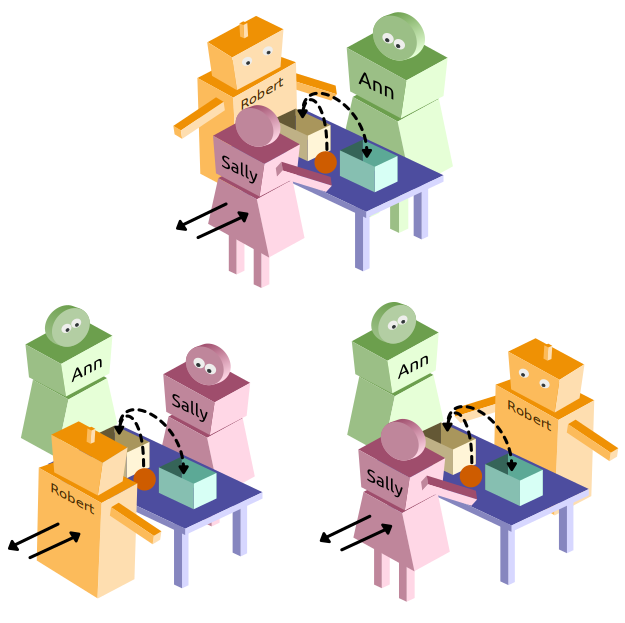
\includegraphics[width=0.6\textwidth]{triadic_false_beliefs}
\end{frame}
}

\imageframe{zoo}

{
    \paper{Frith and Happé {\bf Autism: Beyond "theory of mind"} -- Cognition, 1994]\newline
           [Lemaignan, Dillenbourg {\bf Mutual Modelling in Robotics: Inspirations for the Next Steps} -- HRI 2015}
\begin{frame}{Further investigating socio-cognitive traits}
    \centering
    \begin{tabular}{p{0.45\linewidth}p{0.45\linewidth}}
        \toprule
        {\bf Already in the HRI fridge} & {\bf To buy...} \\
        \midrule
        Instrumental gestures & Expressive gestures \\
        Using person as tool & Using person as receiver of information \\
        Talking about desires and emotions & Talking about beliefs and ideas \\
        Showing "active" sociability & Showing "interactive" sociability \\
        Elicited structured play & Spontaneous pretend play \\
        \bottomrule
    \end{tabular}
        \badge{europe_epfl}
\end{frame}
}


{
    \paper{Frith and Happé {\bf Autism: Beyond "theory of mind"} -- Cognition, 1994]\newline
           [Lemaignan, Dillenbourg {\bf Mutual Modelling in Robotics: Inspirations for the Next Steps} -- HRI 2015}
\begin{frame}{Autistic assets and deficits observed in real life}
    \centering
    \begin{tabular}{p{0.45\linewidth}p{0.45\linewidth}}
        \toprule
        {\bf Assets} & {\bf Deficits} \\
        \midrule
        Instrumental gestures & Expressive gestures \\
        Using person as tool & Using person as receiver of information \\
        Talking about desires and emotions & Talking about beliefs and ideas \\
        Showing "active" sociability & Showing "interactive" sociability \\
        Elicited structured play & Spontaneous pretend play \\
        \bottomrule
    \end{tabular}
        \badge{europe_epfl}
\end{frame}
}

{
    \paper{Verbrugge, {\bf Logic and social cognition}, Journal of Philosophical
    Logic, 2009}
\begin{frame}{In Epistemic Logics: Agreement as $\infty$-order ToM}
    \only<1>{
    \begin{center}
    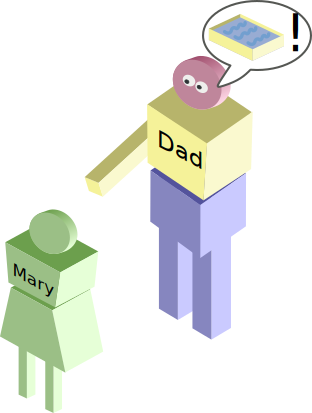
\includegraphics[width=0.4\textwidth]{mutual-agreement.pdf}
    \end{center}
}
\only<2->{
    \begin{center}
    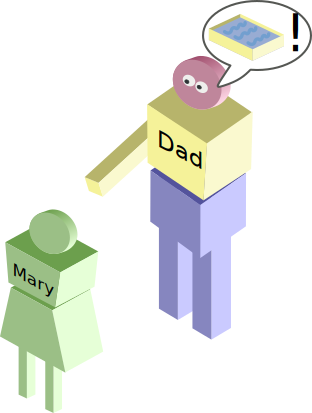
\includegraphics[width=0.2\textwidth]{mutual-agreement.pdf}
    \end{center}

    \uncover<2->{
    Shared knowledge
\[
    \mathsf{EK}_J\varphi \leftrightarrow \bigwedge_{i \in J}\mathsf{K}_i\varphi
\]
}
\uncover<3>{
    Common knowledge 
\[
    \mathsf{CK}_J\varphi \leftrightarrow
\mathsf{EK}_J\varphi \wedge \mathsf{EK}_J\mathsf{EK}_J\varphi \wedge
\mathsf{EK}_J\mathsf{EK}_J\mathsf{EK}_J\varphi \wedge ...
\]
}
}
\end{frame}
}


\begin{frame}{My toolbox to investigate artificial social cognition}
    \begin{itemize}
        \item Symbolic artificial social cognition: \emph{social situation
            assessment}, \emph{mutual task planning}
        \item {\bf Cognitive neurosciences} $\rightarrow$ theories of social
            awareness
        \item Developmental psychology
            \begin{itemize}
                \item Parten's social hierarchy of play
                \item Theory of Mind
                \item socio-cognitive deficits observed in ASD
            \end{itemize}
        \item Modal logics (in particular, epistemic logic) $\rightarrow$
            philosophy of mind
        \item ...
    \end{itemize}
\end{frame}



\section{Back to the question}

\begin{frame}{A model of artificial social cognition}

    I postulate {\bf two stages}:

    \begin{enumerate}
        \item building models of others' minds
        \item exploiting these models to socially act:
            \begin{itemize}
                \item prediction, reading others' intentions
                \item adapting own behaviour, alignment
                \item establish join goals
                \item ultimately, performing joint actions
            \end{itemize}
    \end{enumerate}

    \vspace{2em}
    $\rightarrow$ Social analogs of \emph{perception} \& \emph{action}

\end{frame}

{
    \paper{see discussion in Vernon, {\bf Artificial Cognitive Systems: A Primer} 2014}
\begin{frame}{Cognitivist vs Emergent paradigms}

    ``building'', ``exploiting'', ``reading'', ``establishing''... my terminolgy
    denotes a cognitivist approach (`I, the designer of the system, explicitly implement
    these capabilities')

    \pause
    
    Reformulation in the emergent paradigm:

    \begin{enumerate}
        \item developing internal states \emph{connoting} others' minds
        \item perturbing (influencing) actions synthesis with these states
    \end{enumerate}

    \pause

    Hybrid approaches are possible -- mapping to ``phenomenal experience'' vs
    ``access counciousness''.
\end{frame}
}

\begin{frame}{Sketching a path forward: mentalizing}

    {\bf Hypothesis 1}: Graziano is right: mental representations are snapshots of
    \emph{awareness}, \emph{awareness} being itself a label for the
    \emph{memory-mediated process of attention}.

    \pause

    {\bf Hypothesis 2}: this can be extended to social cognition. \textbf{Modeling one
    other mental representations equates to taking snapshots of their current
    state of awareness}.

    As we do not have direct access to others' process of attention, it has to
    be mediated. Following Graziano, we hypotesise that \textbf{modelling other's
    state of awareness is mediated by one's own attentional system, through
    joint attention mechanisms}.


\end{frame}

{

    \paper{Graziano's Attention Schemata Theory; Desimone and Ducan {\bf Biased Competition
Model of Attention} 1995; Block 1996}

\begin{frame}{In more details}
\footnotesize
    \begin{enumerate} \item<+-> {\bf mental representations} are {\bf snapshots
                of what we are aware of}

        \item<+-> {\bf awareness} is the label we conveniently put on the {\bf
            process of attention}

        \item<+-> attention at time t is the label we put on the set of the {\bf
            activated units} in a (biased) {\bf associative memory network}

        \item<+-> modelling {\bf others’ mental representations} is taking
            snapshots of their own current state of awareness

        \item<+-> modelling other’s state of awareness, \ie their current
            attentional process, is {\bf mediated by one’s own attentional
            system}, typically through {\bf joint attention} mechanisms

        \item<+-> Points 1 to 5 essentially refer to a \emph{phenomenal}
            awareness (a \emph{raw} inner experience). \emph{Phenomenal}
            awareness can be turned into \emph{access consciousness} (the
            abstract, cognitive ability to reflect on the inner experience)

        \item<+-> In robots, \emph{access consciousness} can be mapped to {\bf
            symbolic representations}

    \end{enumerate}


\end{frame}
}

\begin{frame}{What are the gaps?}

    \begin{itemize}

        \item  mental representations are likely not simply instantaneous
            'snapshots' -- even though I could argue that they indirectly embed
            a notion of time and history as they are snapshots of activated
            units in an associative memory network;

        \item equating attention to a set of activated units in a memory network raises
            questions regarding the nature of these units: physical entities? active
            interaction modalities? ...? In particular, the right level of
            abstraction of these units is not immediately clear: the spectrum is
            rather large, from raw perceptual inputs 'à la Tony Morse' to
            high-level units like objects, joint gazing, etc.

        \item the Biased Competition Model of Attention supports interesting bottom-up
            and top-down biasing mechanisms: bottom-up is quite clear (if a unit is
            activated longer/stronger, it biases the resulting attention to this
            unit. Top-down is less clear (but also potentially very interesting
            as it closes the loop between the sub-symbolic and symbolic models):
            how more abstract cognitive process can influence the memory network
            to bias the attention process?

        \item the access to other's mental representations is mediated by one's own
            attentional system: the consequences of this mediation are not immediately
            clear

        \item I conveniently map the split between 'phenomenal consciousness' and
            'access consciousness' respectively to sub-symbolic and symbolic
            computational structures. This need to be better evidenced, if only
            because the frontier between phenomenal and access consciousness is
            all be clear (as pointed by Graziano).

        \item It is not yet clear how the sub-symbolic and symbolic models of the
            different agent co-exist: is each agent a different unit in the same
            associative network?  one associative memory per agent? what about
            the symbolic level?

        \item What is the {\bf motivation}? What social drives?
    \end{itemize}

\end{frame}


\begin{frame}{Sketching a path forward: social behaviours}

    {\bf Hypothesis 3}: together, representations of one's and others' minds are
    \emph{necessary} and \emph{sufficient} for social behaviours to emerge

    {\bf Hypothesis 3'}: representations of one's and others' minds, along with
    a situation (physical and temporal environment), are \emph{necessary} and
    \emph{sufficient} conditions for social behaviours to emerge

    \pause

    How?


\end{frame}

\begin{frame}{What could the model predict?}

    \begin{itemize}

        \item {\bf behavioural alignment} $\rightarrow$ surface alignment and/or
            global alignment $\rightarrow$ the original 'maze' task by Pickering
            and Garrod is certainly relevant here: every time you play the same
            game with the same person, the interaction is more fluid

        \item ability to pass {\bf false-belief tasks}, including
            non-perceptual, non-physical, abstract ones,

        \item {\bf recursive awareness}: \emph{being aware of being aware} -- typically
            evidenced by being able to describe/verbalize its own state of
            awareness 

        \item {\bf 'natural' (\ie emergent) turn-taking}: I 'just' know when it is my
            turn to act

        \item {\bf 'natural' protodeclarative pointing}: I 'just' know when I really
            need to draw your attention on something

        \item {\bf Emergence of Parten's hierarchy?}

    \end{itemize}

\end{frame}

%%%%%%%%%%%%%%%%%%%%%%%%%%%%%%%%%%%%%%%%%%%%%%%%%%%%%%%%%%%%%%%%%
%%%%%%%%%%%%%%%%%%%%%%%%%%%%%%%%%%%%%%%%%%%%%%%%%%%%%%%%%%%%%%%%%
%%%%%%%%%%%%%%%%%%%%%%%%%%%%%%%%%%%%%%%%%%%%%%%%%%%%%%%%%%%%%%%%%
\section{Experimental investigation}

\begin{frame}{An experimental framework for investigation}

    \begin{itemize}
        \item<1-> Typical socio-cognitive tasks are either toy scenarios (\ie do not mirror
            real-world siutation) or simple, constraint tasks that do not
            reflect the complexity \& dynamics of real-world interactions
        \item<2-> $\Rightarrow$ {\bf free play}: richer set of cognitive and
            social dynamics; importance of motivation/drive; forces us to deal
            with uncertain and unexpected situations
        \item<3-> Challenge to isolate behaviours, analyses them (and if we are
            to avoid Wizard-Of-Oz, implementation challenge!)
    \end{itemize}
\end{frame}

\videoframe[0.56]{figs/next/maud-zoe-pilot-edit.mkv}

\begin{frame}{An experimental framework}

    \begin{itemize}
        \item The ``Zoo design'' play situation
        \item {\bf Free play} with the following constraints:
            \begin{itemize}
                \item initial prompt (``Let's build a zoo!'')
                \item limited set of tokens (cubes, Lego animals)
                \item spatially limited playground
            \end{itemize}
        \item<2-> to make it technically tractable with robots, the physical
            playground is {\bf replaced by a large touchscreen} (sandtray): entirely
            skips the difficult problem of perception and manipulation in a
            dense \& cluttered scene
        \item<2-> the touchscreen strictly
            replace the perception of objects on the playground (exports
            ROS TF frames of each object) and their manipulation (receives
            virtual 'touches' from the robot)
        \item<2-> importantly, perception of the partner and of the global scene
            geometry is genuine
    \end{itemize}
\end{frame}

\imageframe[color=black]{next/zoo-activity2}
\imageframe[color=black]{next/zoo-activity}
\videoframe[0.56]{figs/next/zoo-builder-proto-smaller.mkv}


\begin{frame}{Analysis}

    \begin{itemize}
        \item Ballard's (and Anderson's extension) coding of children's free-play interactions
        \item behavioural alignment between partners: for instance, using
            Słowinski's \emph{Individual Motor Signature}
    \end{itemize}
\end{frame}

\section{La route est encore longue}
\begin{frame}{Open questions}

    The most obvious one: {\bf what cognitive model?}

    $\rightarrow$ will draw from hybrid architectures (CLARION), internal
    simulation (HAMMER), sub-symbolic cognitive architecture (ERA)

    ...but not many cognitive architectures model social interactions! (on BICA
    website, about 0 actually!)

    \pause
    
    The second most obvious one: {\bf what are the inputs?} low-level?
    high-level? To reconstruct someone else's attentional state, Graziano suggests:

    \begin{itemize}
        \item gaze direction
        \item facial expression
        \item body language
        \item prior knowledge of person
        \item location of salient objects
    \end{itemize}

\end{frame}

\begin{frame}[plain]{}

    {\bf Thank you!}

    {\bf\tt\scriptsize severin.lemaignan@plymouth.ac.uk}

\end{frame}

\end{document}
